\section{Protocol and reproducibility}
\label{app:protocol}
{\raggedright
Every configuration was fixed in a written protocol addendum before the run it governs; the addenda, scripts and per-seed result files are in the code repository.
Development folds chose checkpoints, mirror averaging and the gate threshold; the official test cases were used for the final scores.
Code is at \url{https://github.com/volcanictv/grasp-instrument-classifier} and the weights, with checksums, at \url{https://huggingface.co/AryanB005/grasp-instrument-pipeline}.\par}
\todo{research repository link for the training and analysis code, if we release it}

\section{Additional results}
\label{app:extra}
\begin{figure}[h]
\floatconts
  {fig:reliability}
  {\caption{Reliability diagrams on the held-out fold, pooled over the three seeds: stated confidence against accuracy in 10 bins; points below the diagonal are overconfident, and the area of a point follows the number of instruments.}}
  {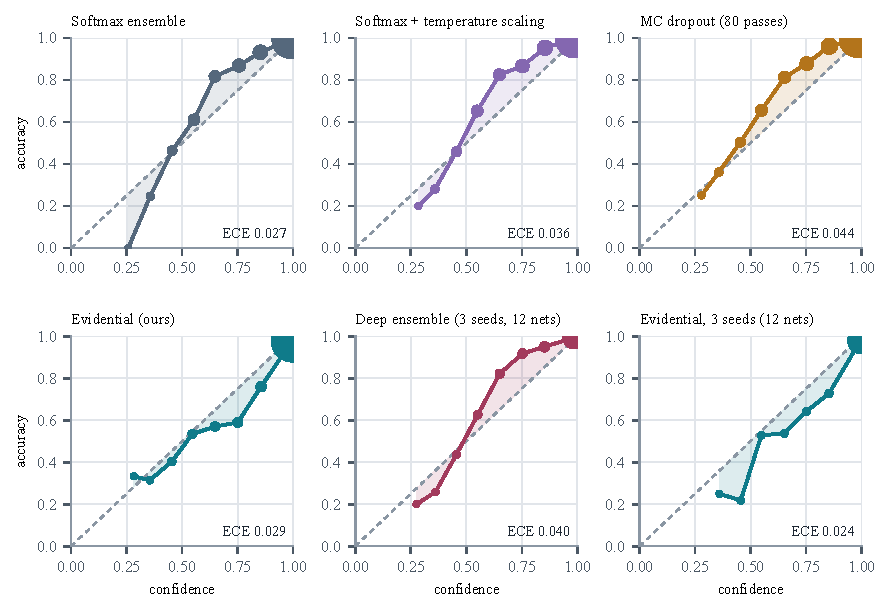
\includegraphics[width=0.9\linewidth]{figures/fig5_reliability.pdf}}
\end{figure}

\begin{table}[h]
\floatconts
  {tab:test-selected}
  {\caption{The configuration with the test-selected share (833 of 2,861 instruments, 29\%), mean of three seeds, with the 95\% bootstrap interval over the five test cases.}}
  {\small\begin{tabular}{lrrr}
  \toprule
  & \bfseries mIoU & \bfseries IoU & \bfseries mcIoU\\
  \midrule
  Refined, 29\% of the instruments & 87.37 & 86.22 & 78.33\\
  95\% interval & 86.9 to 88.2 & 85.6 to 87.1 & 76.3 to 79.8\\
  \bottomrule
  \end{tabular}}
\end{table}

\begin{table}[h]
\floatconts
  {tab:cost}
  {\caption{Cost of each stage in GFLOPs (multiply-adds, matmul, convolution and attention, counted with PyTorch's FLOP counter on one forward pass) with parameters, and the time measured on one A100. The frame stage is shared by the instruments of a frame (2.54 on average).}}
  {\footnotesize\setlength{\tabcolsep}{4pt}\begin{tabular}{lrrr}
  \toprule
  \bfseries Stage & \bfseries GFLOPs & \bfseries Params (M) & \bfseries A100 (s)\\
  \midrule
  SAM2.1-large, one pass & 913 & 224 & \\
  SAM2.1-tiny, one pass & 148 & 39 & \\
  SAM3, one pass & 2,810 & 458 & \\
  Classifier, four members, one crop & 12.5 & 50 & \\
  SAM2-large tracking, 21 frames & 25,321 & 224 & \\
  \midrule
  Single pass, per instrument & 2,953 & & 1.2 (per frame)\\
  Refining one instrument & 25,584 & & 6.1\\
  \bottomrule
  \end{tabular}}
\end{table}
The single pass uses SAM2-large and SAM3 on a frame and its mirror image; with SAM2-tiny alone it costs 0.13\,TFLOPs per instrument and gives 82.13 mIoU against 83.47.

\begin{table}[h]
\floatconts
  {tab:control}
  {\caption{Control: the keyframe's own mask applied unchanged to the $\pm10$ neighbouring frames (static box) against SAM2-large tracking, 29\% of the instruments refined, mean of three seeds.}}
  {\small\begin{tabular}{lrrr}
  \toprule
  \bfseries Frames & \bfseries mIoU & \bfseries IoU & \bfseries mcIoU\\
  \midrule
  single pass & 83.47 & 81.07 & 69.94\\
  static box & 75.84 & 72.81 & 63.55\\
  SAM2-large tracking & 87.37 & 86.22 & 78.33\\
  \bottomrule
  \end{tabular}}
\end{table}

\begin{table}[h]
\floatconts
  {tab:ladder}
  {\caption{Steps of the pipeline (mean of three classifier seeds, 29\% of the instruments refined).}}
  {\small\begin{tabular}{lrrr}
  \toprule
  \bfseries Step & \bfseries mIoU & \bfseries IoU & \bfseries mcIoU\\
  \midrule
  SAM2 fine-tuned segmenter & 86.34 & 85.31 & 77.59\\
  + SAM3 in the segmenter & 86.78 & 85.72 & 77.90\\
  + classifier trained on tracker-style crops & 87.11 & 85.97 & 78.19\\
  + segmenters trained on all training cases & 87.37 & 86.22 & 78.33\\
  \bottomrule
  \end{tabular}}
\end{table}
SAM3 raises the mask IoU against the ground truth from 0.900 to 0.906, and tracker-style crops help most on the Prograsp Forceps (IoU 61 to 67) at some cost on the Large Needle Driver (90 to 86); steps of 0.3 or less are within the seed spread.

\begin{figure}[h]
\floatconts
  {fig:qualitative}
  {\caption{Test frames: ground truth, the single-pass labels and the labels after refinement, on the same masks (coloured by class; $*$ sent to refinement; green: class fixed; red: wrong). Every instrument is right in 78.5\% of the test frames after the single pass and in 89.9\% after refinement (headline seed). Rows one and two: refinement fixes a Bipolar Forceps and a Suction Instrument; row three: nothing needed refining; row four: a Bipolar Forceps that both labellings get wrong.}}
  {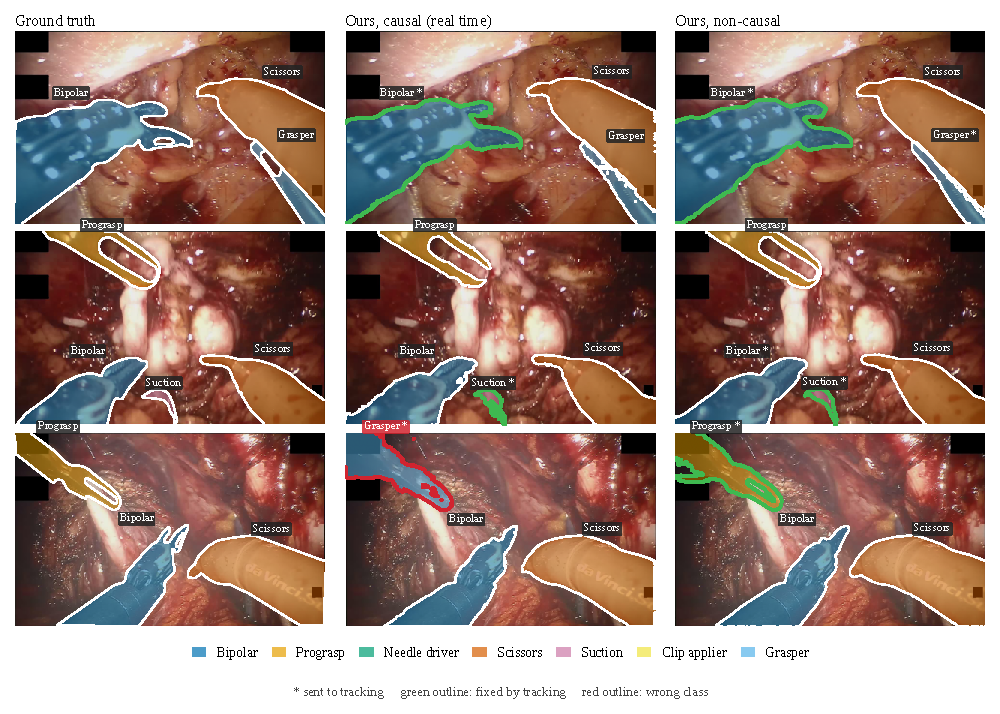
\includegraphics[width=0.78\linewidth]{figures/fig3_qualitative.pdf}}
\end{figure}

\paragraph{Clipping to the given box.}
The given boxes are the tight extent of the ground-truth masks, so clipping a predicted mask to its box uses the true mask extent and helps only when boxes are given; as an oracle variant it moves the pipeline at 29\% from 87.37, 86.22 and 78.33 to 87.61, 86.46 and 78.59 (mIoU, IoU, mcIoU); no result in the paper uses it.
\todo{per-case scores and leave-one-case-out ranges}

\section{Implementation details}
\label{app:impl}
\todo{optimiser, learning rates, epochs, batch sizes and augmentations for the segmenters and the four classifier members; GPU and software versions; time measurement protocol (one NVIDIA A100-PCIE-40GB, 4 CPU cores, PyTorch 2.8.0 with CUDA 12.6, frame copying into the video predictor excluded, 20 timed keyframes)}
